\Case{plain-pen-and-relative-tail}{
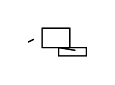
\begin{tikzpicture}
  \draw (-8pt,2pt) -- (-6pt,3pt) -- plot[ybar] coordinates {(2pt,7pt)(8pt,-3pt)} -- ++(1pt,2pt);
  \draw (-8pt,2pt) -- (-6pt,3pt) plot[ybar] coordinates {(2pt,7pt)(8pt,-3pt)} -- ++(1pt,2pt);
\end{tikzpicture}}

\Case{rotated-pen-and-relative-tail}{
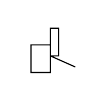
\begin{tikzpicture}
  \draw (-8pt,2pt) -- plot[ybar,rotate=90] coordinates {(2pt,7pt)(8pt,-3pt)} -- ++(1pt,2pt);
\end{tikzpicture}}

\Case{ybar-default}{

\begin{tikzpicture}
  \draw[line width=2pt] plot[ybar] coordinates {(2pt,7pt)(9pt,-4pt)(-3pt,0pt)};
\end{tikzpicture}}

\Case{xbar-default}{
\begin{tikzpicture}
  \draw plot[xbar] coordinates {(-7pt,2pt)(4pt,9pt)(0pt,-3pt)};
\end{tikzpicture}}

\Case{fixed-source-width-and-shift}{
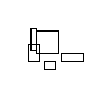
\begin{tikzpicture}[bar width=8pt,bar shift=1pt]
  \draw plot[ybar,/pgf/bar width=4pt,/pgf/bar shift=-2pt] coordinates {(1pt,6pt)(7pt,-3pt)};
  \draw[xbar,bar shift=3pt] plot coordinates {(-2pt,5pt)(8pt,4pt)};
  \draw plot[ybar=99pt] coordinates {(12pt,3pt)};
\end{tikzpicture}}

\Case{negative-and-unitless-width}{
\begin{tikzpicture}
  \draw plot[xbar,bar width=-4,bar shift=2] coordinates {(5pt,1pt)(-4pt,7pt)};
  \draw plot[ybar,bar width=0pt,bar shift=-1] coordinates {(2pt,-6pt)(8pt,3pt)};
\end{tikzpicture}}

\Case{ybar-interval-default}{
\begin{tikzpicture}
  \draw plot[ybar interval] coordinates {(2pt,7pt)(9pt,-4pt)(-3pt,50pt)};
\end{tikzpicture}}

\Case{xbar-interval-default}{
\begin{tikzpicture}
  \draw plot[xbar interval] coordinates {(-7pt,9pt)(3pt,2pt)(80pt,11pt)};
\end{tikzpicture}}

\Case{interval-width-and-shift}{
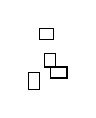
\begin{tikzpicture}[bar width=80pt,bar shift=-30pt]
  \draw plot[ybar interval,bar interval width=.5,/pgf/bar interval shift=.25]
    coordinates {(2pt,5pt)(10pt,-4pt)(-2pt,8pt)};
  \draw plot[xbar interval,/pgf/bar interval width=-.5,bar interval shift=1.25]
    coordinates {(5pt,2pt)(-4pt,10pt)(8pt,-2pt)};
\end{tikzpicture}}

\Case{coincident-interval-and-relative-tail}{
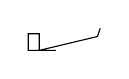
\begin{tikzpicture}
  \draw (2pt,4pt) -- plot[xbar interval] coordinates {(6pt,3pt)(-4pt,3pt)(20pt,9pt)}
    -- +(1pt,-1pt) -- ++(2pt,2pt);
\end{tikzpicture}}

\Case{empty-and-singleton}{
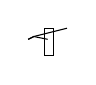
\begin{tikzpicture}
  \draw plot[ybar] coordinates {};
  \draw plot[xbar interval] coordinates {(60pt,70pt)};
  \draw (-6pt,2pt) -- (-4pt,3pt) -- plot[ybar interval] coordinates {(7pt,4pt)} -- ++(1pt,2pt);
  \draw (-6pt,2pt) -- (-4pt,3pt) plot[xbar] coordinates {} -- ++(1pt,2pt);
  \draw plot[xbar] coordinates {(3pt,1pt)};
\end{tikzpicture}}

\Case{fixed-file-gaps}{
\begin{tikzpicture}[x=2pt,y=3pt]
  \draw (-5pt,2pt) -- plot[xbar,bar width=2pt] file {observations.table} -- ++(1,1);
\end{tikzpicture}}

\Case{interval-file-gaps}{
\begin{tikzpicture}[x=2pt,y=3pt]
  \draw (-5pt,2pt) -- plot[ybar interval] file {observations.table} -- ++(1,1);
  \draw plot[xbar interval,bar interval width=.5] file {observations.table};
\end{tikzpicture}}

\Case{transformed-basis-and-interval}{
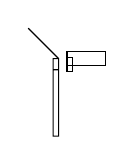
\begin{tikzpicture}[x={(4pt,1pt)},y={(-2pt,3pt)},xshift=7pt]
  \draw (1,0) -- plot[xbar interval,rotate=90,xscale=-2,bar interval width=.5]
    coordinates {(1,1)(3,-1)(-2,2)} -- ++(1,2);
  \draw plot[xbar,xshift=2pt,yscale=-.5] coordinates {(1,1)(3,-1)};
\end{tikzpicture}}

\Case{rounded-fixed-and-interval}{
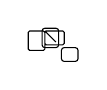
\begin{tikzpicture}
  \draw[rounded corners=1pt] plot[ybar,bar width=6pt] coordinates {(2pt,7pt)(9pt,-5pt)};
  \draw plot[xbar interval,rounded corners=.5pt] coordinates {(7pt,1pt)(-6pt,6pt)(2pt,-1pt)}
    -- ++(2pt,3pt);
\end{tikzpicture}}

\Case{scoped-and-adjacent-overrides}{
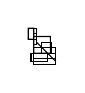
\begin{tikzpicture}[xbar,bar width=6pt,bar shift=2pt]
  \begin{scope}[ybar interval,bar interval width=.5]
    \draw plot coordinates {(1pt,4pt)(8pt,-3pt)(-4pt,1pt)};
    \draw plot[/tikz/xbar,bar width=2pt] coordinates {(1pt,4pt)(8pt,-3pt)};
  \end{scope}
  \draw plot coordinates {(1pt,4pt)(8pt,-3pt)};
  \draw plot[ybar,sharp plot] coordinates {(1pt,4pt)(8pt,-3pt)}
    -- plot[/tikz/xbar interval] coordinates {(-2pt,5pt)(3pt,9pt)}
    plot[ybar=false] coordinates {(1pt,6pt)};
\end{tikzpicture}}

\Case{every-plot-and-expression}{
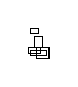
\begin{tikzpicture}[x=3pt,y=2pt,every plot/.style={ybar interval,bar interval width=.5}]
  \draw plot[samples at={-1,2,0,3}] (\x,{\x*\x-2});
  \draw plot[xbar,bar width=2pt] coordinates {(1,3)(2,-1)};
\end{tikzpicture}}

\Case{dimensional-math}{
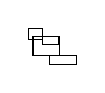
\begin{tikzpicture}
  \draw plot[ybar,bar width={2*1mm+4pt},bar shift={1pt-.5mm}] coordinates {(2pt,7pt)(8pt,-3pt)};
  \draw plot[xbar interval,bar interval width={1/2},bar interval shift={1/4+1/2}]
    coordinates {(-5pt,2pt)(6pt,10pt)(3pt,4pt)};
\end{tikzpicture}}

\Case{constant-zero-streams}{
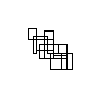
\begin{tikzpicture}
  \begin{scope}
    \pgfplotxzerolevelstreamconstant{-3pt}
    \pgfplotyzerolevelstreamconstant{2pt}
    \draw plot[ybar,bar width=4pt] coordinates {(3pt,5pt)(8pt,-4pt)};
    \draw plot[xbar,bar width=4pt] coordinates {(3pt,5pt)(-6pt,9pt)};
    \draw plot[ybar interval] coordinates {(3pt,1pt)(8pt,-4pt)(2pt,3pt)};
    \draw plot[xbar interval] coordinates {(1pt,3pt)(-4pt,8pt)(3pt,2pt)};
  \end{scope}
  \draw plot[ybar] coordinates {(3pt,5pt)};
  \draw plot[xbar] coordinates {(3pt,5pt)};
\end{tikzpicture}}

\Case{nonzero-winding-cancellation}{

\begin{tikzpicture}
  \fill[nonzero rule] plot[ybar interval] coordinates {(1pt,7pt)(9pt,7pt)(1pt,50pt)};
  \fill[nonzero rule] plot[xbar,bar width=2pt] coordinates {(6pt,13pt)(6pt,13pt)};
\end{tikzpicture}}

\Case{dash-origin}{
\begin{tikzpicture}
  \draw[dashed] plot[ybar,bar width=5pt] coordinates {(1pt,8pt)(7pt,-4pt)};
  \draw[dashed] plot[xbar interval,xscale=-1] coordinates {(5pt,2pt)(-3pt,11pt)(1pt,3pt)};
\end{tikzpicture}}
